
\minitoc 

% =======================================================================================================
% Introduction 

L'objectif de ce chapitre est d'être capable d'organiser efficacement un flot d'objects 
dans un réseau. Par exemple, on souhaite amener le maxium de camions d'un point A à un point B 
en passant par certaines routes. De même, on souhaiterai savoir comment router efficacement le 
plus de paquets dans un réseau informatique. 

Tout ces problèmes se généralisent en ce que l'on appelle la \emph{recherche de flot maximal
dans un graphe orienté}. Nous allons ici définir proprement ce genre de problème, donner des conditions 
d'existence de flot maximal et proposer des algorithmes pour les construire. 


% =======================================================================================================
% Rappels sur les graphes 

\section{Rappels sur les graphes}

Pour représenter une structure de réseau (routier, informatique, etc...), on utilise les graphes. 
Ce cours fait donc suite à celui sur la théorie des graphes enseigné en licence. Effectuons quelques rappels. 

\begin{definition}[Graphe Orienté]
    On appelle graphe orienté un couple d'ensembles finis $G = (X,E)$ où $X = \{1, \dots, n\}$ représente les sommets du graphe 
    et $E = \{ (x_i, y_j), \dots \}$, $ x_i, y_j \in X$ l'ensemble ordonné des arrêtes du graphe. 
    Pour un graphe orienté, les notions de graphe simple et multiraphe sont les même que pour le cas non orienté.
\end{definition}


\begin{example}[Graphes et leur représentation gravarphique]
    Soient $G_1$ et $G_2$ deux graphes, en voici une représentation :
    \begin{figure}[h]
        \centering
        \begin{minipage}{0.45\textwidth}  % Première image dans 45% de la largeur de la page
          \centering
          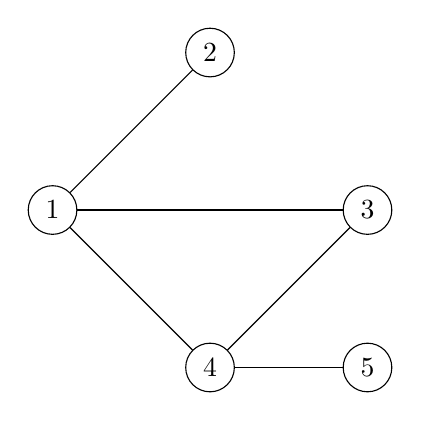
\begin{tikzpicture}[scale=1]
            % Déclaration des sommets avec des cercles
            \node[draw, circle] (1) at (0,0) {1};
            \node[draw, circle] (2) at (2,2) {2};
            \node[draw, circle] (3) at (4,0) {3};
            \node[draw, circle] (4) at (2,-2) {4};
            \node[draw, circle] (5) at (4,-2) {5};
      
            % Ajout des arêtes (non orientées)
            \draw (1) -- (2);
            \draw (1) -- (3);
            \draw (1) -- (4);
            \draw (4) -- (5);
            \draw (3) -- (4);
          \end{tikzpicture}
          \caption{Graphe non orienté}
          \label{fig:non-oriente}
        \end{minipage}%
        \hfill % Ajoute de l'espace flexible entre les deux images
        \begin{minipage}{0.45\textwidth}  % Deuxième image dans 45% de la largeur de la page
          \centering
          \begin{tikzpicture}[->,>=stealth',shorten >=1pt,auto,node distance=2cm,thick,scale=1]
            % Déclaration des sommets avec des cercles
            \node[draw, circle] (1) at (0,0) {1};
            \node[draw, circle] (2) at (2,2) {2};
            \node[draw, circle] (3) at (4,0) {3};
            \node[draw, circle] (4) at (2,-2) {4};
            \node[draw, circle] (5) at (4,-2) {5};
      
            % Ajout des arêtes orientées
            \draw[->] (1) -- (2);
            \draw[->] (1) -- (3);
            \draw[->] (4) -- (1);
            \draw[->] (2) -- (4);
            \draw[->] (3) -- (5);
          \end{tikzpicture}
          \caption{Graphe orienté}
          \label{fig:oriente}
        \end{minipage}
      \end{figure}
\end{example}

\begin{definition}[Voisinnage]
    Le voisinnage d'un sommet $x$ de $G$ est l'ensemble des sommets $y$ de $G$ tels qu'il existe une arrête entre $x$ et $y$ dans $G$.
    On le note $V(x)$.
\end{definition}

\begin{remark}
    Si $x$ est dans le voisinnage de $y$, on dira que $x$ est adjascent à $y$ et inversement.
\end{remark}

\begin{definition}[Degré]
    Le degré d'un sommet $x$ de $G$ est le cardinal du voisinnage $x$. On le note $d(x)$.
    Un sommet de voisinnage nul est dit \emph{isolé} et un sommet de voisinnage égal à 1 est dit \emph{pendant}.
\end{definition}

\begin{definition}[Voisinnage entrant et sortant]
    Soit $G$ un graphe orienté et $x$ un sommet de $G$. On définit deux types de voisinnages :
    \begin{itemize}
        \item \emph{Voisinnage entrant :} noté $V^-(X)$ est l'ensemble des prédécesseurs de $x$.
        \item \emph{Voisinnage sortant :} noté $V^+(X)$ est l'ensemble des successeurs de $x$.
    \end{itemize}
    On définira comme précédemment le degré sortant et le degré entrant d'un sommet $x$.
\end{definition}


\begin{definition}[Chaine]
    On appelle chaine de $G = (X,E)$ de longueur $n$ toute suite alternée de sommets et d'arrêtes de $G$ telle que :
        \[ c = (x_0, a_1, x_1, \dots, a_n, x_n), \text{  telle que } \forall i \in \llbracket 1, n \rrbracket, a_i = (x_{i-1}, x_i) \]
    Ici, $n$ représente le nombre d'arrêtes de la chaine. Dans le cas d'un graphe simple, on notera les chaines de la façon suivante :
        \[ c = (x_0, \dots, x_n) \quad \text{ou} \quad c = x_0 - x_1 - \dots - x_n \] 
    Dans le cas des graphes orientés, on notera une chaîne simplement avec les arrêtes dont elle est constituée : 
        $$ c = (u_1, \dots, u_n), \forall i \in \llbracket 1, n \rrbracket u_i \in E $$
\end{definition}

\begin{definition}[Accessibilité]
    Soit $G = (X,E)$ un graphe. On a :
    \begin{itemize}
        \item Soient $x$ et $y$ deux sommets de $G$. On dit que $y$ est accessible à partir de $x$ s'il existe une chaine joignant $x$ et $y$ dans $G$.
        \item $G$ est dit \emph{connexe} ssi $ \forall x \in X, \forall y \in X$, $y$ est accessible à partir de $x$.
        \item L'accessibilité est un relation d'équivalence entre les sommets. 
        
        Ses classes d'équivalences sont les composantes connexes de $G$.
    \end{itemize}
\end{definition}

\begin{definition}[Chaîne Simple]
    Une chaine est \emph{simple} si elle ne passe pas deux fois par la même \emph{arrête} et elle est dite \emph{élémentaire} 
    si elle ne passe pas deux fois pas le même \emph{sommet}.
    On remarquera facilement qu'une chaîne élémentaire est simple.
\end{definition}

\begin{definition}[Cycle]
    Un cycle de $G$ est une chaine simple dont le départ et l'arrivée sont le même sommet. Un cycle est donc de la forme :
        \[ c = x_0 - x_1 - \dots - x_{n-1} - x0 \] 
\end{definition}

\begin{theorem}[Propriétés des cycles et chaînes]
    Soit $G$ un graphe à $ n \in \N$ sommets. 
    \begin{itemize}
        \item Toute chaine élémentaire a une longueur inférieure à $n-1$
        \item Toute cycle élémentaire a une longueur inférieure à $n$
        \item De toute chaîne, on peut en extraire une chaîne élémentaire.
    \end{itemize}
\end{theorem}

% =======================================================================================================
% Cycle et flots

\section{Cycle et flot}

Définissons maintetant la notion de flot dans un cas général. 

% \begin{definition}[Graphe Pondéré]
%     On appelle \emph{graphe pondéré} tout graphe $G = (X,E)$ auquel on a ajouté une \emph{fonction de poids} : 
%         \[ 
%             \mu : 
%                 \begin{cases}
%                     E \longrightarrow \R \\
%                     u = (x,y) \longmapsto \alpha 
%                 \end{cases}
%         \] 
%     qui, à chaque arrête du graphe lui associe un réel. On notera alors : 
%             \[ G := (X,E, \mu) \] 
% \end{definition}

% \begin{example}[Graphe orienté]
%     Soit $G_1 = (X,E, \mu)$ le graphe orienté pondéré suivant : 
%     \begin{figure}[h]
%         \centering
%         \begin{tikzpicture}[->,>=stealth',shorten >=1pt,auto,node distance=2cm,thick,scale=1]
%             % Déclaration des sommets avec des cercles
%             \node[draw, circle] (1) at (0,0) {1};
%             \node[draw, circle] (2) at (2,2) {2};
%             \node[draw, circle] (3) at (4,0) {3};
%             \node[draw, circle] (4) at (2,-2) {4};
%             \node[draw, circle] (5) at (4,-2) {5};

%             % Ajout des arêtes orientées avec poids
%             \draw[->] (1) -- (2) node[midway, above left] {3}; 
%             \draw[->] (1) -- (3) node[midway, above right] {5};
%             \draw[->] (4) -- (1) node[midway, left] {2};
%             \draw[->] (2) -- (4) node[midway, below left] {4};
%             \draw[->] (3) -- (5) node[midway, below right] {1};
%         \end{tikzpicture}
%         \caption{Graphe orienté pondéré}
%     \end{figure}

%     On peut décrire l'application $ \mu : E \longrightarrow \R$ comme suit : 
%         $$ \mu(1,2) = 3, \quad \mu(1,3) = 5, \quad \mu(2,4) = 4 $$ 
%         $$ \mu(3,5) = 1, \quad \mu(4,1) = 2 $$ 
% \end{example}

\begin{definition}[Vecteur de chaîne]
    Soit $c = (u_1, \dots, u_n)$ une \emph{chaîne élémentaire} dans 
    un graphe orienté $ G = (X, E)$ tel que $ |E| = n $ et d'arcs $ u_i$. 
    On appelle \emph{vecteur de chaîne} l'application $ \varphi$ associée à $c$ telle que : 
        $$ 
            \varphi : 
                \begin{cases}
                    E \longrightarrow \Z \\ 
                    u_i \longmapsto 
                        \begin{cases}
                            1 \text{ si } u_i \text{ est dans le sens de } c \\ 
                            -1 \text{ si } u_i \text{ n'est pas dans le sens de } c \\ 
                            0 \text{ si } u_i \text{ n'est pas dans } c \\
                            \end{cases}
                \end{cases}
        $$
    On la note en général $ \varphi = ( \varphi(u_1), \varphi(u_2), \dots, \varphi(u_n)) \in \Z^n$. 
\end{definition}

Venons en maintetant à la définition phare de ce chapitre : 

\begin{definition}[flot]
    Soit $G = (X, E, c)$ un graphe orienté. On appelle \emph{flot} dans $G$ tout vecteur de 
    cycle $ \varphi$ de $G$ qui vérifie la loi de Kirchoff : 
        $$ \forall x \in X, \quad \sum_{ u_i \in \omega^-(\{X\})} \varphi(u_i) = \sum_{u_i \in \omega^+(\{X\})} \varphi(u_i) $$
    Et on note $ \varphi^i = \varphi(u_i)$ le \emph{flot} de l'arrête $u_i$. 
\end{definition}

\begin{remark}
    Un flot est donc un chaîne élémentaire d'un graphe orienté dont, pour chaque noeud, la somme des flots 
    sortants est égale à la somme des flots entrants. 
\end{remark}

\begin{example}
    Soit $G$ le graphe suivant :
    \begin{figure}[h]
        \centering 
        \begin{tikzpicture}[->,>=stealth',shorten >=1pt,auto,node distance=2cm,thick,scale=1]
            % Déclaration des sommets avec des cercles
            \node[draw, circle] (1) {1};
            \node[draw, circle, right of=1, above of=1] (2) {2}; 
            \node[draw, circle, right of=2, below of=2] (3) {3}; 
            \node[draw, circle, right of=2] (4) {4}; 
            \node[draw, circle, right of=4, below of=4] (5) {5}; 

            % Ajout des arêtes orientées avec poids
            \draw[->] (1) -- (2) node[midway, above] {$u_1$}; 
            \draw[->] (1) -- (3) node[midway, above] {$u_2$}; 
            \draw[->] (2) -- (4) node[midway, above] {$u_4$};
            \draw[->] (3) -- (2) node[midway, above] {$u_3$};
            \draw[->] (4) -- (3) node[midway, above] {$u_5$};
            \draw[->] (4) -- (5) node[midway, above] {$u_6$};
            \draw[->] (5) -- (3) node[midway, above] {$u_7$};     
            % \draw[->] (1) -- (2) node[midway, above left] {3}; 
            % \draw[->] (1) -- (3) node[midway, above right] {5};
            % \draw[->] (4) -- (1) node[midway, left] {2};
            % \draw[->] (2) -- (4) node[midway, below left] {4};
            % \draw[->] (3) -- (5) node[midway, below right] {1};
        \end{tikzpicture}
        \caption{flot dans un graphe}
    \end{figure}
    Le vecteur $ \varphi_1 = (2, -2, 1, 3, 4, -1, 1)$ est un flot de $G$. 
    Le vecteur $ \varphi_2 = (0,0,0,0,1, -1,1)$ est aussi un flot. 
    Soit $ v = 2 \varphi_1 + 3 \varphi_2$, c'est aussi un flot de $G$. 
\end{example}

\begin{prop}[flots]
    Soit $G = (X,E, c)$ un graphe tel que $|E| = n$, alors : 
    \begin{itemize}
        \item Le vecteur null de $\Z^n$ est un flot de $G$. 
        \item Toute combinaison linéaire de flots de $G$ est aussi un flot de $G$. 
        \item Tout vecteur cyclique de $G$ est un flot de $G$. 
    \end{itemize}
\end{prop}

\begin{proposition}[Loi de Kirchoff généralisée]
    Soit $G = (X, E, c)$ et $A \subset E$ non vide. Un chaîne $ \varphi$ est un flot de $G$ ssi : 
        $$ \sum_{u \in \omega^-(A)} \varphi(u) = \sum_{u \in \omega^+(A)} \varphi(u) $$
\end{proposition}

% =======================================================================================================
% Flot dans un réseau de transport 

\section{Flot et coupure}

\subsection{Flot maximal dans un réseau}

Dans cette section, nous revenons à notre problème de départ en définissant la notion de graphe de transport. 
Graphes dans lesquels nous chercherons à construire des flots maximaux. 

\begin{definition}[Réseau de Transport]
    Un \emph{réseau de transport} est un graphe orienté pondéré $ R = (X, E, c)$ qui contient : 
    \begin{itemize} 
        \item un sommet {sans prédécesseur} appelé \emph{source} (noté $s$). 
        \item  un sommet {sans fils} appelé \emph{puit} (noté $t$). 
        \item $ c$ est une fonction qui, à chaque arc, lui associe sa capacité, notée $c$ : 
            \[ 
                c : 
                    \begin{cases}
                        E \longrightarrow \R \cup \{\infty\} \\
                        u = (x,y) \longmapsto c(u) 
                    \end{cases}
            \] 
        \item un arc fictif de $t$ à $s$ doté d'une capacité infinie, appelé \emph{arc retour}. 
    \end{itemize}
\end{definition}

\begin{example}
    Voici un exemple de réseau de transport : 
    \begin{figure}[h]
        \centering 
        \begin{tikzpicture}[->,>=stealth',shorten >=1pt,auto,node distance=2cm,thick,scale=1]
            % Déclaration des sommets avec des cercles
            \node[draw, circle] (1) {s};
            \node[draw, circle, right of=1, above of=1] (2) {2}; 
            \node[draw, circle, right of=2, below of=2] (3) {3}; 
            \node[draw, circle, right of=2] (4) {4}; 
            \node[draw, circle, right of=4, below of=4] (5) {t}; 

            % Ajout des arêtes orientées avec poids
            \draw[->] (1) -- (2) node[midway, above] {$(5)$}; 
            \draw[->] (1) -- (3) node[midway, above] {$(2)$}; 
            \draw[->] (2) -- (4) node[midway, above] {$(4)$};
            \draw[->] (3) -- (2) node[midway, above] {$(4)$};
            \draw[->] (4) -- (3) node[midway, above] {$(3)$};
            \draw[->] (4) -- (5) node[midway, above] {$(5)$};
            \draw[->] (5) -- (3) node[midway, above] {$(3)$};     
            \draw[dashed, bend left] (5) edge (1) node[below right] {$(\infty)$};  
        \end{tikzpicture}
        \caption{Réseau de Transport}
    \end{figure}
\end{example}

\begin{definition}[Flot compatible]
    Un \emph{flot compatible} sur un réseau $ R = (X,E, c)$ tel que $ |E| = n$ 
    est un vecteur $ \varphi \in \mathbb{Z}^n$ qui vérifie :
    \begin{itemize}
        \item (\textbf{Conservation de Kirchhoff}) pour tout $x \in X \setminus \{s, t\}$ 
        (hors source $s$ et puits $t$), on a :
        $$ \sum_{u \in \omega^+(x)} \varphi(u) = \sum_{u \in \omega^-(x)} \varphi(u) $$
        où $\omega^+(x)$ (resp. $\omega^-(x)$) est l'ensemble des arcs sortants (resp. entrants) de $x$.
        \item (\textbf{Compatibilité avec les capacités}) :
        $$ \forall u \in E, \quad 0 \leqslant \varphi(u) \leqslant c(u). $$
    \end{itemize}
    La \emph{valeur} du flot, notée $v(\varphi)$, est définie par :
    $$ v(\varphi) := \sum_{u \in \omega^+(s)} \varphi(u) - \sum_{u \in \omega^-(s)} \varphi(u), $$
    c'est-à-dire le flux net sortant de la source (équivalent au flux net entrant dans le puits).
    Enfin, on dit qu'un arc $u$ est \emph{saturé} si $\varphi(u)=c(u)$.
\end{definition}


\begin{definition}[Flot maximal]
    Un \emph{flot maximal} d'un réseau est un flot compatible qui maximise la valeur 
    $v(\varphi)$ parmi tous les flots compatibles du réseau.
\end{definition}

\subsection{Théorème de Coupure minimale}

Pour construire un flot maximal dans un réseau, nous avons besoin d'un peu de théorie. 

\begin{definition}[Coupure et cocycle]
    Soit $R = (X, E, c)$ un réseau de flot, où $X$ est l'ensemble des sommets, $E$ l'ensemble des arêtes
    et $c : E \to \mathbb{R}^+$ la fonction de capacité. 
    
    Une \emph{coupure} $ct$ séparant $s$ de $t$ est un couple $(A, X \setminus A)$ tel que :
    \[
        s \in A, \qquad t \notin A.
    \]
    
    L'ensemble des arêtes de la coupure, noté $\mathrm{arcs}(ct)$, est le \emph{cocycle sortant} de $A$ :
    \[
        \mathrm{arcs}(ct) = \omega^+(A) := \{ u = (i,j) \in E \mid i \in A, j \in X \setminus A \}.
    \]
\end{definition}

\begin{definition}[Capacité d'une coupure]
    La \emph{capacité} d'une coupure $ct$ est la somme des capacités de ses arêtes :
    \[
        \mathrm{capa}(ct) := \sum_{u \in \omega^+(A)} c(u).
    \]
\end{definition}

\begin{remark}
    Retrirer tout les arcs du cocycle d'une coupure revient à couper tous les chemins de $s$ vers $t$. 
    Donc les arrêtes sortantes d'une coupure sont exactement celles qu'il faut couper pour déconnecter 
    $s$ de $t$. 
\end{remark}

\begin{theorem}[Flot et coupure minimale]
    Pour tout flot compatible $ \varphi$ et pour toute coupure $ct$ d'un réseau $R$, on a : 
        $$ v( \varphi) \leqslant \mathrm{capa}(ct) $$ 
\end{theorem}